\documentclass[10pt]{article}
\usepackage{graphicx}
\usepackage[margin=1.5cm]{geometry}
\usepackage{amsmath}
\def\brcurs{{\mbox{$\resizebox{.16in}{.08in}{
\includegraphics{BoldR}}$}}}
\def\brcurs{{\mbox{$\resizebox{.16in}{.08in}{
\includegraphics{ScriptR}}$}}}

\begin{document}
\twocolumn

\title{Tuesday Warm-up: Vector Algebra and Calculus Review}
\author{Prof. Jordan C. Hanson}

\maketitle

\section{Review: Differential Vector \\ Calculus}

\begin{enumerate}
\item Calculate the gradient for the following functions: (a) $f(x,y) = x^2 + y^2$. (b) $g(x,y) = \sqrt{1-x^2+y^2}$, for $x^2 + y^2 \leq 1$. (c) Where are the local minima and/or maxima?  \\ \vspace{2cm} 
\item Consider the separation vector $\brcurs = \mathbf{r} - \mathbf{r}'$. (a) Show that
\begin{equation}
\brcurs = (x-x')\hat{\mathbf{x}}+(y-y')\hat{\mathbf{y}}+(z-z')\hat{\mathbf{z}}
\end{equation}
(b) Calculate $\nabla \cdot \brcurs$.  The result should be a \textit{scalar.} \\ \vspace{2cm}
\item Calculate $\nabla \times \brcurs$. Justify the result using symmetry arguments.  \\ \vspace{2cm}
\item (a) Calculate the \textit{Laplacian} of $h(x,y)$, $\nabla^2 h$, in exercise 1.  Explain the sign of the result. (b) What would be the sign of $\nabla^2 g$ at locations other than the origin? \\ \vspace{2cm}
\end{enumerate}

\section{Review: Integral Vector Calculus}

\begin{figure}
\centering
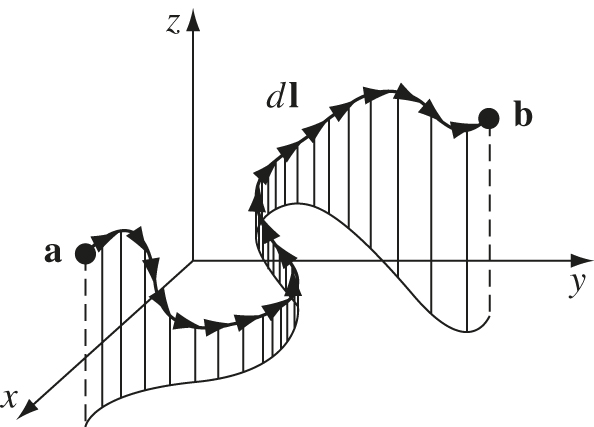
\includegraphics[width=0.3\textwidth]{figures/1_20.jpg}
\caption{\label{fig:1} The work required to move a system through an external net force is given by the \textit{line integral.}  The dot product of each $d\mathbf{l}$ with $\mathbf{F}$ gives $dW$.}
\end{figure}

\begin{enumerate}
\item Recall the definition of \textit{work} from mechanics (Fig. \ref{fig:1}):
\begin{equation}
W = \int \mathbf{F} \cdot d\mathbf{l}
\end{equation}
(a) Let $\mathbf{F} = 10\hat{\mathbf{x}}$, and let the path be restricted to the x-axis. If a particle is released from the origin, what work is done on it by $\mathbf{F}$ from (0,0) to (10,0)? \\ \\ \\
(b) Let $f(x,y)$ be a differentiable scalar function.  The \textit{Fundamental Theorem of Calculus} for gradients states that
\begin{equation}
\int_{\mathbf{a}}^{\mathbf{b}} (\nabla f) \cdot d\mathbf{l} = f(\mathbf{b})-f(\mathbf{a})
\end{equation}
Suppose $f(x,y) = (1/2)k(x^2 + y^2)$.  Evaluate the line integral of $\mathbf{F}(x,y) = -k(x\hat{\mathbf{x}}+y\hat{\mathbf{y}}) = -k\mathbf{r}$ on (i) the straight path from (0,0) to (1,0), (ii) the straight path from (0,0) to (0,1), and the circular path with radius 1, beginning and ending at (1,0). \\ \\ \\ \\ \\
\item Suppose $\mathbf{f}(\mathbf{r},\mathbf{r}') = \brcurs$.  (a) Compute the divergence. (b) Perform the volume integral of the result over the sphere of radius 1, centered at the origin. (b) Perform the surface integral of $\mathbf{f}$ over the sphere of radius 1, centered at the origin.
\end{enumerate}

\end{document}
